\documentclass[12pt]{article}

\usepackage{mathtools}
\usepackage[a4paper,margin=1in,bottom=1.5in,showframe]{geometry}
\usepackage{tikz}
\usepackage{pgfplots}

\definecolor{darkgreen}{RGB}{0,64,0}


\tikzset{small dot/.style={fill=black, circle,scale=0.2}}
%\tikzset{every pin/.style={}}

\begin{document}

\begin{figure}[!ht]
\centering
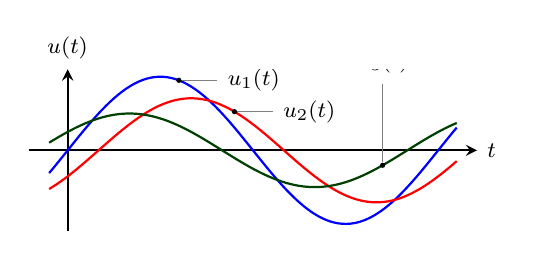
\begin{tikzpicture}[font=\footnotesize]

    \begin{axis}[
        width=0.6\textwidth,
        height=0.3\textwidth,
        domain=-0.1*pi:2.1*pi,
        axis lines=middle,
        ticks=none,
        thick,
        samples=101,
%        axis line style={shorten >=-10pt, shorten <=-10pt},
%        enlargelimits,
        enlarge x limits=0.05,
        enlarge y limits=0.05,
        xlabel style={
                anchor=west,
                at={(ticklabel* cs:1.00)},
%                xshift=10pt
            },
        xlabel=$t$,
        ylabel style={
            anchor=south,
            at={(ticklabel* cs:1.0)},
%            yshift=10pt
        },
        ylabel=$u(t)$
    ]
    \addplot[blue] {sin(deg(x))}; 
    \addplot[red] {0.707*sin(deg(x)-30)}; 
    \addplot[darkgreen] {0.5*sin(deg(x)+30)}; 
    
%    \node[small dot, pin=0:{$u_1(t)$}] at (axis description cs:0.35,0.9) {};
    \node[small dot, pin=0:{$u_1(t)$}] at (axis cs:0.6*pi,{sin(0.6*180)}) {};
    \node[small dot, pin=0:{$u_2(t)$}] at (axis cs:0.9*pi,{0.707*sin(0.9*180-30)}) {};
    \node[small dot, pin={[pin distance=1cm]90:{$u_3(t)$}}] at (axis cs:1.7*pi,{0.5*sin(1.7*180+30)}) {};
    
    \end{axis}
\end{tikzpicture}
\end{figure}

\begin{equation}
\begin{split}
u_1(t) &= \sin (2\pi t)\\
u_2(t) &= \tfrac{1}{2}\sqrt{2}\sin\left(2\pi t-\tfrac{1}{6}\pi\right)\\
u_2(t) &= \tfrac{1}{2}\sin\left(2\pi t+\tfrac{1}{6}\pi\right)
\end{split}\end{equation}


\end{document}